%!TEX root = thesis.tex

\section{Principles and Methods}
To understand motion illustration design and production, we surveyed related literature, studied collected examples, and interviewed individuals who create such illustrations.

\subsection{Design Principles}
Cutting~\cite{cutting_representing_2002} argues that superimposing vector-like lines, often called ``actions lines'', on an image satisfies four important criteria: it evokes a feeling of motion, the object undergoing motion is clearly represented without deformation, the direction of motion is clear, and the magnitude of motion is conveyed with reasonable precision. To complement this metaphoric representation, Cutting also argues for the more literal method of multiple stroboscopic images, which satisfies all criteria except clear motion direction. McCloud~\cite{mccloud_understanding_1994} provides further arguments and examples for using these methods in the field of comic illustration, and notes communication benefits when they are combined.

To examine how professional illustrators use motion lines and stroboscopic images, we gathered examples from sources like user manuals, gesture-based games, safety guides, % (e.g., for airplane safety or weight training),
illustration compendia (e.g.,~\cite{mijksenaar1999open}) and how-to books (e.g.,~\cite{greenberg2012sketching}).
%
We found Cutting's notion of vector-like lines are almost always rendered with an arrowhead % with of a clear head at the end of a line tracing the motion path.
in a variety of styles (heads, weights, colors) with strokes typically two-dimensional, smooth, and offset to avoid occluding the object.
Stroboscopic images can be overlapping or spatially distributed, and change in transparency or shading to convey time.
The most common style for depicting the object undergoing motion is a simplified black-and-white contour drawing, but filled silhouettes and flat-shaded colour can also be found -- using full color photographic detail is rare.
%
By carefully removing extraneous details, such techniques help readers focus on only the salient motion information.

\subsection{Interviews: Methods Used In the HCI Community}
Conveying movement for interaction is common in HCI publications. We found 100 motion illustrations in 58 recent papers.
%
To understand current creation methods, we conducted video interviews with six Human-Computer Interaction researchers with experience creating motion illustrations.

\subsubTitleBold{Findings}
% in 3 categories: tools and creation process, motivations, and struggles
% Several authors emphasized the importance of concision and focus: they introduced important concepts via illustrations with unnecessary details excluded, like faces, clothing, and backgrounds. Establishing a consistent visual style was important to reuse graphic elements. %, especially for operating mobile devices.
%
All interviewees used a similar methodology to create motion illustrations: they took still photographs of people performing actions, traced outlines using Adobe Photoshop (4/6) or Illustrator (2/6), then added graphic annotations to convey motion. %One interviewee with design expertise sometimes drew illustrations from scratch.
%All interviewees mentioned the importance of iterating illustrations. Often preliminary versions were created for an early draft and refined later.
% 4 of the 6 interviewees used Photoshop, while 2 used Illustrator; 3 solely used a mouse while 3 used a stylus as a main input device.
%
All mentioned that it was time-consuming to set up scenes and poses, take and trace photos, then add details like arrow placement while maintaining a consistent style. Typical creation times were estimated between 10 minutes to a few hours.
They also noted how difficult it was to make adjustments: changing the pose or viewpoint essentially meant starting over again with new source photos and re-tracing.
Yet, identifying the best pose and viewpoint ahead of time is difficult and it often took several iterations to yield an illustration suitable for publication.

\begin{figure}[t]
  \centering
  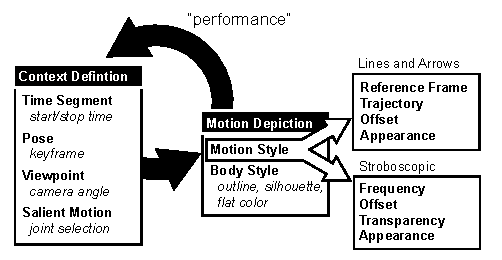
\includegraphics[width=0.7\columnwidth]{\demodraw/fig/designdimensions}
  \caption{Canonical authoring workflow consisting of a Motion Definition task then a Motion Depiction task. Design decisions associated with a task are shown in bold with design parameters in italics.}
  \label{fig:designspace}
\end{figure}

\subsection{Design Space Goals and Workflow}

Based on the observations above, we derive a canonical workflow to motivate our system's central design goal.
Authors face two primary illustration tasks (Figure~\ref{fig:designspace}):
\textit{defining the motion} for portraying movements like the view of the body and salient moving joints;
and \textit{exploring a style of motion depiction} by choosing styles like lines-and-arrows or stroboscopic, then adjusting related style parameters.
These tasks and the underlying design parameters are highly interdependent, so authoring motion illustrations is necessarily an iterative process.
This means that changes to one task parameter often leads to re-evaluating and changing the other.
The problem with current methods, is that movements are mostly ``performed'' using a time-consuming process of taking photos and manually tracing them.
%
Therefore, the central design goal of our system is to make motion definition low effort and iterative via interactive demonstrations.

Designing a system to capture interactive demonstrations of \textit{any} body movement also poses an input challenge.
Since  body movements form the demonstration itself, also issuing application commands with a body gesture introduces ambiguity.
Using a hand held device, touch screen, or any conventional input is not ideal since performing requires open space and full freedom of movement.
For these reasons, we use a multi-modal voice and gesture interaction style traced back to Bolt's Put-That-There~\cite{Bolt:1980:PutThatThere}. Like Bolt, we use voice for commands like \iquote{start} and \iquote{stop} with body movements providing command parameters in the form of the recorded demonstration, and for setting parameter context with utterances like \iquote{one, two, three, four} to label step-by-step segments.
